\section{Multiplatformní framework}

Vývoj mobilních aplikací je dle \cite{wepc_video_game_statistics} na vzestupu.
To přináší nároky na vydavatele a vývojáře k rychlejší tvorbě mobilních
aplikací a her. 
Aplikace pro mobilní zařízení se běžně vytvářejí pomocí programovacích jazyků,
které jsou úzce spjaty s mobilními zařízeními.
Příkladem takového programovacího jazyka je jazyk Java,
který se použivá pro vývoj nativních aplikací v platformě Android.
Tyto jazyky mají úzkou podporu pro vývoj na daných zařízeních,
včetně přístupu k hardwarovému rozhraní (kamera, senzory, \dots{}),
jak uvádí zdroj \cite{dashmagazine_mobile_frameworks}. 

\begin{figure}[ht!]
    \centering
    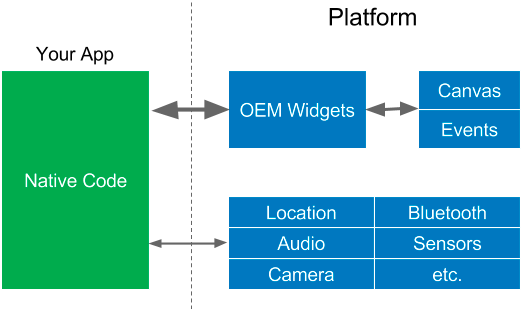
\includegraphics[width=\linewidth]{assets/technology-research/framework/platform_sdk.png}
    \caption{Schéma frameworku specifického pro platformu \todo{do vektoru} \cite{hackernoon_flutter}}
    \label{fig:framework_platform}
\end{figure}

Snahu urychlit vývoj mobilních aplikací řeší také mobilní frameworky.
Tyto frameworky jsou tvořeny většinou stejnou společností,
která také vytváří danou platformu
a jsou publikování jako \emph{Software Development Kit} (dále jen SDK).
\cite{dashmagazine_mobile_frameworks}
Pro platformu Android je vývíjeno Android SDK,
spolu s podpůrnými programy jako integrované vývojové prostředí
(dále jen IDE) a emulátory.
Tyto frameworky jsou díky jejich úzkému propojení a plné kompatabilitě
považovány za rychlé,
avšak mnohdy vyžadují speciální znalosti pro konkrétní platformu.
Právě cílení výhradně na danou platformu je největší nevýhoda těchto typů
frameworků.
Architekturu těchto frameworků představuje obrázek \ref{fig:framework_platform}.

Další snahou pro ještě rychlejší a snadnější vývoj aplikací jsou frameworky
s podporou multiplatformnosti a tedy cílením na více platforem.
\cite{hackernoon_flutter}
To může být pouze cílení na mobilní platformy,
ale dokonce také i cílení na web, osobní počítače, \dots{}
Tyto frameworky podporují populární jazyky,
umožňují sdílet kód mezi jednotlivými platformami
a v závislosti na architektuře se blíží rychlostí výsledných aplikací
k aplikacím psaných nativními jazyky.
Pomocí těchto technologií lze tedy vyvíjet aplikace pohodlně, rychle
a benefitem \uv{zadarmo} je podpora multiplatformnosti vyvíjené aplikace.
\cite{dashmagazine_mobile_frameworks}

\begin{figure}[ht!]
    \centering
    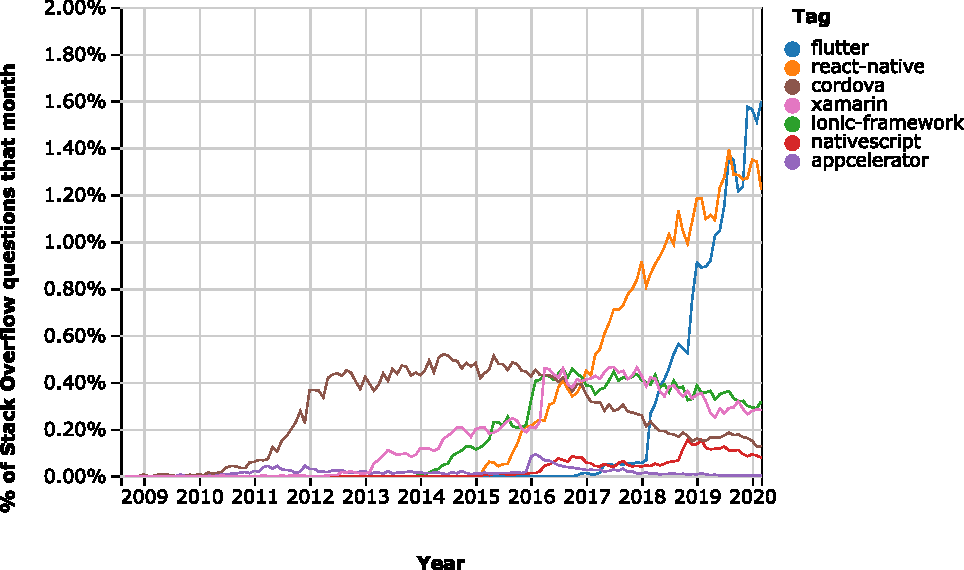
\includegraphics[width=\linewidth]{assets/technology-research/framework/popularity.pdf}
    \caption{Vývoj trendu multiplatformních frameworků
    \cite{framework_popularity}}
    \label{fig:framework_popularity}
\end{figure}

V následujících sekcích je vybráno a popsáno několik multiplatformních
frameworků.
Tyto frameworky byly vybrány na základě trendů \cite{framework_popularity}
na síti Stack Overflow.
Na obrázku \ref{fig:framework_popularity} lze vidět reprezentace těchto trendů,
ve kterých lze vyčíst,
jak se trend pro daný jazyk vyvíjí v čase.
Nejvíce populární na této síti je tedy framework Flutter,
který překonal popularitu frameworku React Native,
avšak oba frameworky si udržují dlouhodobý růst.
Ostatní frameworky si trend udržují,
nebo jim dokonce klesá.

\subsection{Ionic}

\begin{figure}[ht!]
    \centering
    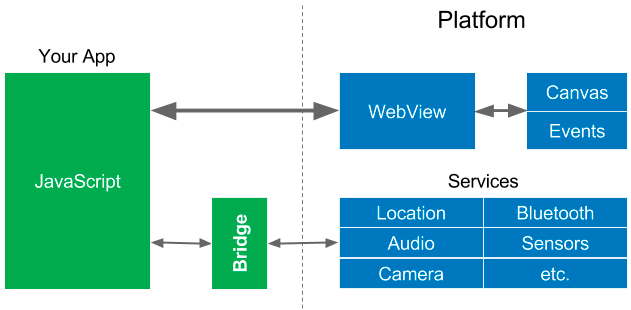
\includegraphics[width=\linewidth]{assets/technology-research/framework/webview.png}
    \caption{Schéma architektury s WebView \todo{do vektoru} \cite{hackernoon_flutter}}
    \label{fig:framework_webview}
\end{figure}

První multiplatformní frameworky začaly pro multiplatformnost využívat WebView.
\cite{hackernoon_flutter}
Tyto frameworky aplikaci vykreslují pomocí webových technologií
a komunikaci s hardwarovým rozhraním řeší pomocí speciálního komunikačního
mostu.
Taková architektura je vidět na obrázku \ref{fig:framework_webview}.
Z tohoto obrázku jde vidět,
jak moc oddělená je 

Jedním z představitelů těchto frameworků je i framework Ionic,
který je stále
--- dle trendů z obrázku \ref{fig:framework_popularity} ---
značně využívaný i v dnešní době.
Framework Ionic využívá jazyky jako HTML, CSS a JavaScript,
a jde v něm vytvořit aplikaci pro mobilní platformy Android a iOS.
Významnou výhodou je,
že díky využití mobilních technologií,
které se používají naprosto shodně jako při vývoji webových aplikací,
se nemusí vývojáři učit nové technologie a přístupy k vývoji,
čímž se také celý proces zrychlí.
Důsledkem používání webových technologií jsou ale i jejich nevýhody,
zejména nižší výkon. \cite{dashmagazine_mobile_frameworks}

S frameworkem Ionic lze využít také frontend knihovny a frameworky. \cite{ionic}
Příkladem jsou knihovny a frameworky React, Angular či Vue.
Součástí je také knihovna komponent UI,
které se automaticky přizpůsobí dané platformě.
Součástí jsou také podpůrné konzolové nástroje pro vytváření, produkování a
testování aplikace.

\subsection{React Native}

Další přístup k vývoji multiplatformních aplikací představuje framework
React Native.
Tento framework využívá pomocí komunikačního mostu nativní komponenty platformy
díky vzorům z reaktivního programování zjednodušuje celkový vývoj.
\cite{hackernoon_flutter}
Framework je založen na populární webové knihovně ReactJs.
\cite{dashmagazine_mobile_frameworks}
Jelikož framework nepoužívá nativní komponenty platformy,
a tedy ani WebView,
jsou aplikace produkované tímto frameworkem rychlejší.
Pro popis UI je používán vlastní jazyk založený na XML, nazývaný JSX.

\begin{figure}[ht!]
    \centering
    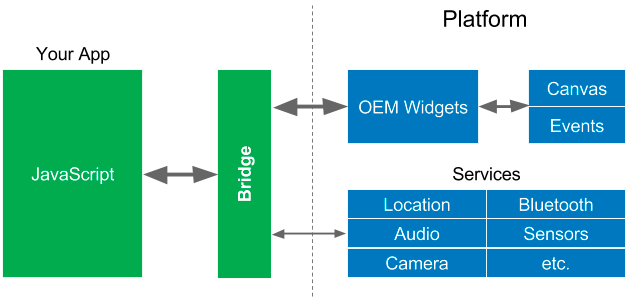
\includegraphics[width=\linewidth]{assets/technology-research/framework/react_native.png}
    \caption{Schéma architektury frameworku React Native \todo{do vektoru} \cite{hackernoon_flutter}}
    \label{fig:framework_react_native}
\end{figure}

Framework React Native obsahuje \emph{hot reloading},
což je vlastnost,
která umožní vidět všechny změny ihned po jejich změně,
bez zbytečně zdlouhavého procesu sestavování celé aplikace.
K dispozici je také velká škála komponent,
včetně velkého množství komponent od vývojářů třetí strany, 
které mohou vývojáři volně používat.
\cite{dashmagazine_mobile_frameworks}

Framework byl vytvořen v roce 2015 \cite{hackernoon_flutter}
společností Facebook,
která jej od té doby spravuje.
Za zmíňku stojí populární aplikace \cite{react_native},
které framework využívají,
kterými jsou například mobilní aplikace Facebook, Instagram, Skype, Discord
a mnoho dalších.

Na obrázku \ref{fig:framework_react_native} lze vidět schéma architektury
frameworku React Native.
Jak lze z obrázku vyčíst,
tato architektura,
oproti architektuře s WebView,
komunikuje s platformou kompletně přes komunikační most pomocí jazyku
JavaScript.

\subsection{Flutter}

Posledním frameworkem je Flutter,
který je vyvíjený společností Google.
Tento framework je nejmladším z představených frameworků,
avšak dle trendů z obrázku \ref{fig:framework_popularity} se jim minimálně
snadno vyrovná.  
Framework Flutter přistupuje k multiplatformnosti jinak,
než ostatní mobilní frameworky.
Nejenže tento framework nevyužívá programovací jazyk JavaScript,
což samo o sobě přináší řadu výhod,
ale také přesouvá starost s vykreslováním z platformy na framework
\cite{hackernoon_flutter},
jak lze vidět na obrázku s reprezentací architektury
\ref{fig:framework_flutter},
a také se plně kompiluje do nativního kódu.
\cite{dashmagazine_mobile_frameworks}
Podporované nejsou pouze mobilní platformy Android a iOS,
ale také platformy web
--- momentálně ve verzi beta ---
a desktop
--- momentálně ve verzi alfa.

\begin{figure}[ht!]
    \centering
    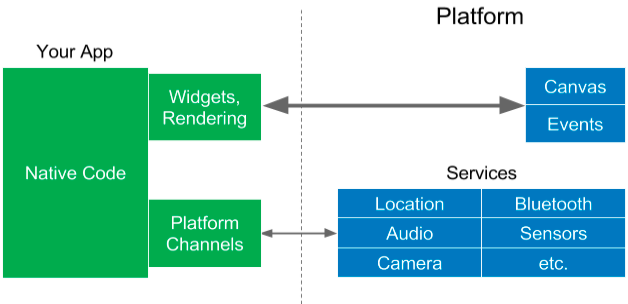
\includegraphics[width=\linewidth]{assets/technology-research/framework/flutter.png}
    \caption{Schéma architektury frameworku Flutter \todo{do vektoru} \cite{hackernoon_flutter}}
    \label{fig:framework_flutter}
\end{figure}

Framework Flutter využívá programovací jazyk Dart,
který umožňuje jak kompilaci \emph{ahead of time} (dále jen AOT),
tak i kompilaci \emph{just in time} (dále jen JIT).
\cite{hackernoon_flutter}
Těmito schopnostmi kompilace do nativního ARM kódu je framework schopen
nemít žádný komunikační most mezi platformou a procesorem,
což umožňuje tvořit rychlejší a výkonější aplikace.
Aplikace mohou dosahovat až 120 snímků za vteřinu.
\cite{dashmagazine_mobile_frameworks}
Díky možnostem kompilace JIT je také framework schopen poskytnout
\emph{hot reload},
který umožní velmi rychle provádět změny stavů aplikace zatímco je spuštěna.
Vydání aplikace jsou vždy kompilovány naopak AOT kompilací,
která produkuje velmi rychlou a výkonou aplikaci.
\cite{hackernoon_flutter}

I přes ne zrovna dlouhou dobu,
za kterou je framework Flutter dostupný,
existuje řada aplikací,
které tento framework využívají.
Za zmíňku stojí například aplikace Google Ads, Baidu, Hamilton a Reflecty.
\cite{flutter}

Tento framework využívá sice widgety (komponenty UI),
které vypadají jako nativní komponenty pro danou platformu \cite{flutter},
avšak všechny tyto widgety implementuje a udržuje pro vlastní vykreslovací
engine Skia,
taktéž od společnosti Google.
Engine Skia je známý 2D grafický engine,
který je využíván například v projektech jako Google Chrome \cite{skia}.

\subsubsection*{Princip frameworku }

Framework Flutter je ve svém principu velmi jednoduchý.
Jak je uvedeno v dokumentaci frameworku Flutter:
\todo{\emph{\uv{Everything’s a widget}}} \cite{flutter_technical_overview}
Oproti ostatním frameworkům,
které dělí aplikaci do několika vrstev,
obsahuje framework Flutter widgety jako základní stavební bloky pro všechno.
Widgety jsou kompozicí spojovány a společně utváří celek, aplikaci.
Každý widget zdědí vlastnosti z jeho rodiče v podobě kontextu,
se kterým může dále samotný widget pracovat.
\cite{flutter_technical_overview}

Pro skladbu widgetů je upřednosťnována kompozice před rozšířením.
Kombinací vhodných widgetů jsou prvky aplikace uspořádány, ostylovány,
transformovány, \dots{}
Například widget \mintinline{dart}|Padding| přidá okolo widgetu odsazení,
widget \mintinline{dart}|Row| uspořádá widgety--potomky do řádku,
zatímco widget \mintinline{dart}|Column| uspořádá widgety--potomky do sloupce.
\cite{flutter_technical_overview}

\begin{figure}[ht!]
    \centering
    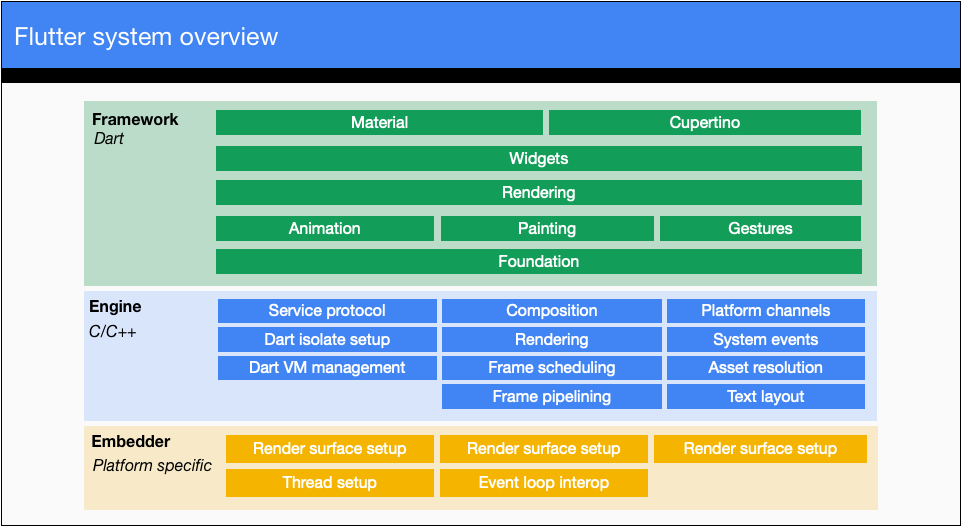
\includegraphics[width=\linewidth]{assets/technology-research/framework/flutter_overview.png}
    \caption{Vrstvy frameworku Flutter \todo{do vektoru; oříznout?} \cite{flutter_technical_overview}}
    \label{fig:flutter_layers}
\end{figure}

Na obrázku \ref{fig:flutter_layers} lze vidět uspořádání frameworku do vrstev
architektury.
Samotný framework je rozdělen do části frameworku samotného na úrovni widgetů
--- které píšou vývojář aplikací v jazyce Dart ---,
enginu, který ovládá framework na nižší urovni,
kompozici widgetů, jejich vykreslování atp.,
--- ten je řešen v programovacích jazycích C a C++ ---
a vrstvě zaměřené na specifickou platformu.
\cite{flutter_technical_overview}

Pokud se widget potřebuje měnit na základě dynamických faktorů,
jako je například interakce uživatele nebo tok dat,
je tento widget označován jako \emph{stateful} (widget se stavem) a je
reprezentovaný třídou \mintinline{dart}|StatefulWidget|.
V opačném případě je widget označován jako \emph{stateless} a je 
reprezentovaný třídou \mintinline{dart}|StatelessWidget|,
která má stav neměnný.
Každý stateful widget má proměnlivý stav \mintinline{dart}|State|
a kdykoli je stav změněn,
je potřeba zavolat metodu \mintinline{dart}|setState()|,
která způsobí signalizaci frameworku,
že je widget notno překreslit s novým stavem.
\cite{flutter_technical_overview}

\subsubsection*{Další platformy}

Framework Flutter momentálně vyvíjí \cite{flutter_web} také podporu pro
další platformy jako jsou platformy web a desktop.
Tyto platformy jsou zatím podporovány pro produkci,
avšak dle obrázku \ref{fig:flutter_layers_web} lze vidět,
že framework Flutter je navržen vhodně k tomu,
aby tato a další úsilí podpořil.
Spodní specifické vrstvy platformy jsou vyměněny za vykreslování pomocí
webových technologií,
což v budoucnu umožní vytvářet aplikace nejen pro platformy Android a iOS,
ale i již zmíněný web a desktop. 

\begin{figure}[ht!]
    \centering
    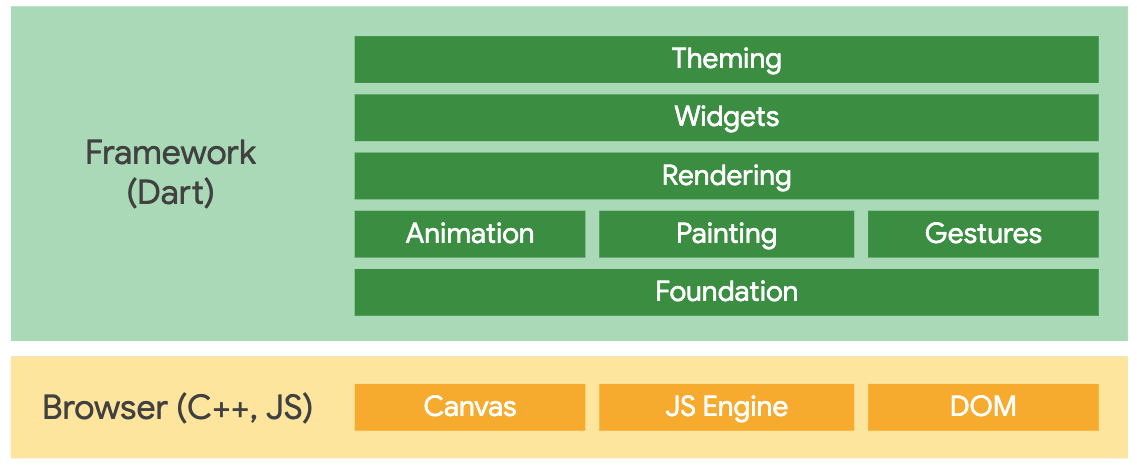
\includegraphics[width=\linewidth]{assets/technology-research/framework/flutter_overview_web.png}
    \caption{Vrstvy frameworku Flutter pro platformu web \todo{do vektoru} \cite{flutter_web}}
    \label{fig:flutter_layers_web}
\end{figure}

\subsection{Zhodnocení}

Jak je již vidět z obrázku \ref{fig:framework_popularity},
nejpopulárnější multiplatformní frameworky jsou frameworky Flutter a
React Native.
Přičemž framework Flutter je v porovnání s frameworkem React Native relativně
stále nový.
I přes to má ale dlouhodobě strmější růst v trendu.

Trend frameworku Ionic dlouhodobě stagnuje, až klesá,
a navíc kvůli již zmiňovaným nevýhodám
--- zejména díky architektuře ---
není až tolik vhodný pro vývoj nových aplikací,
s předpokladem pro dlouhodobější udržitelnost. 

Framework React Native je velmi populární a nabízí skvělé výhody.
Tento framework je však moc spjat s webovými technologiemi
a je nutné využívat komunikační most,
což přináší menší rychlostní i výkonostní nevýhody.
Framework Flutter oproti tomu přináší spoustu výhod,
a jak lze vidět z obrázku \ref{fig:framework_flutter},
tak také zaručuje svou architekturou stejné zobrazení aplikace na všech
verzích operačních systémů dané platformy,
díky vlastnímu vykreslování.
Oba frameworky jsou zajisté vhodné pro vývoj nové aplikace s důrazem na
udržitelnost a rozšiřitelnost,
avšak framework Flutter převyšuje svými výhodami,
a proto bude v praktické části práce využit právě framework Flutter.
